\section{Desenvolvimento}

\subsection*{3.1 Análise visual}

Foram recolhidos dados de amostra para:

- vibração nos eixos X, Y e Z

- movimento circular no eixo Z

- movimento de rotação em torno de um ponto fora do objeto no eixo Y. (Gira e volta)

A aquisição de dados foi feita num período de 50ms.

Nas figuras abaixo vemos os dados recolhidos. Em cada imagem temos 6 gráficos referentes respectivamente à aceleração 3 eixos e giroscópio nos 3 eixos.
Podemos também ver que tivemos etapas de resolução do movimento e etapas de repouso.


\begin{figure}[H]
    \center
    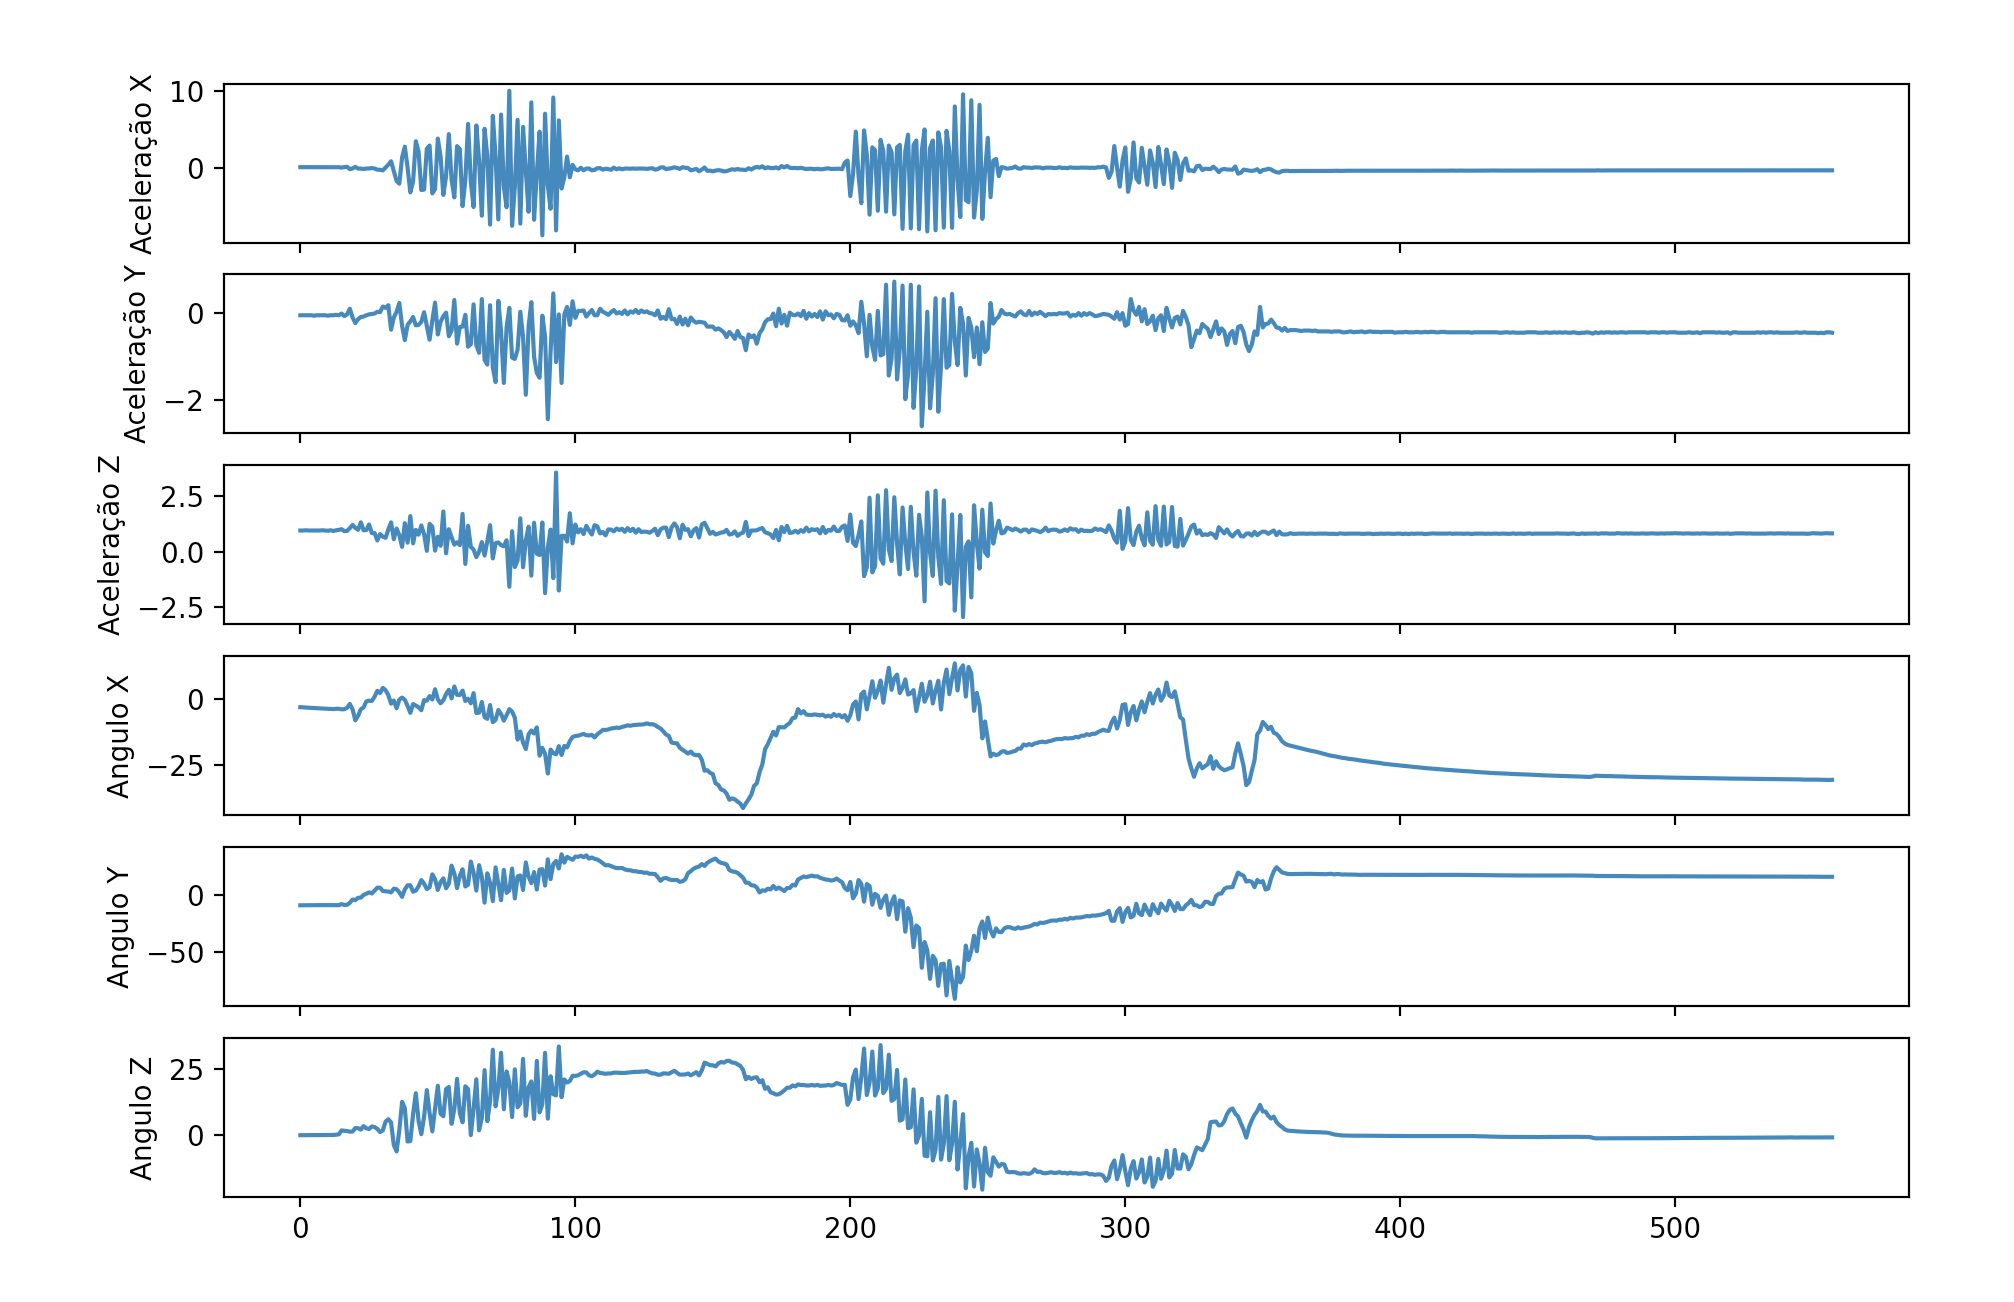
\includegraphics[width=7cm]{images/VibracaoX.png}
    \label{img6}
    \caption{Vibração no eixo X}
\end{figure}

\begin{figure}[H]
    \center
    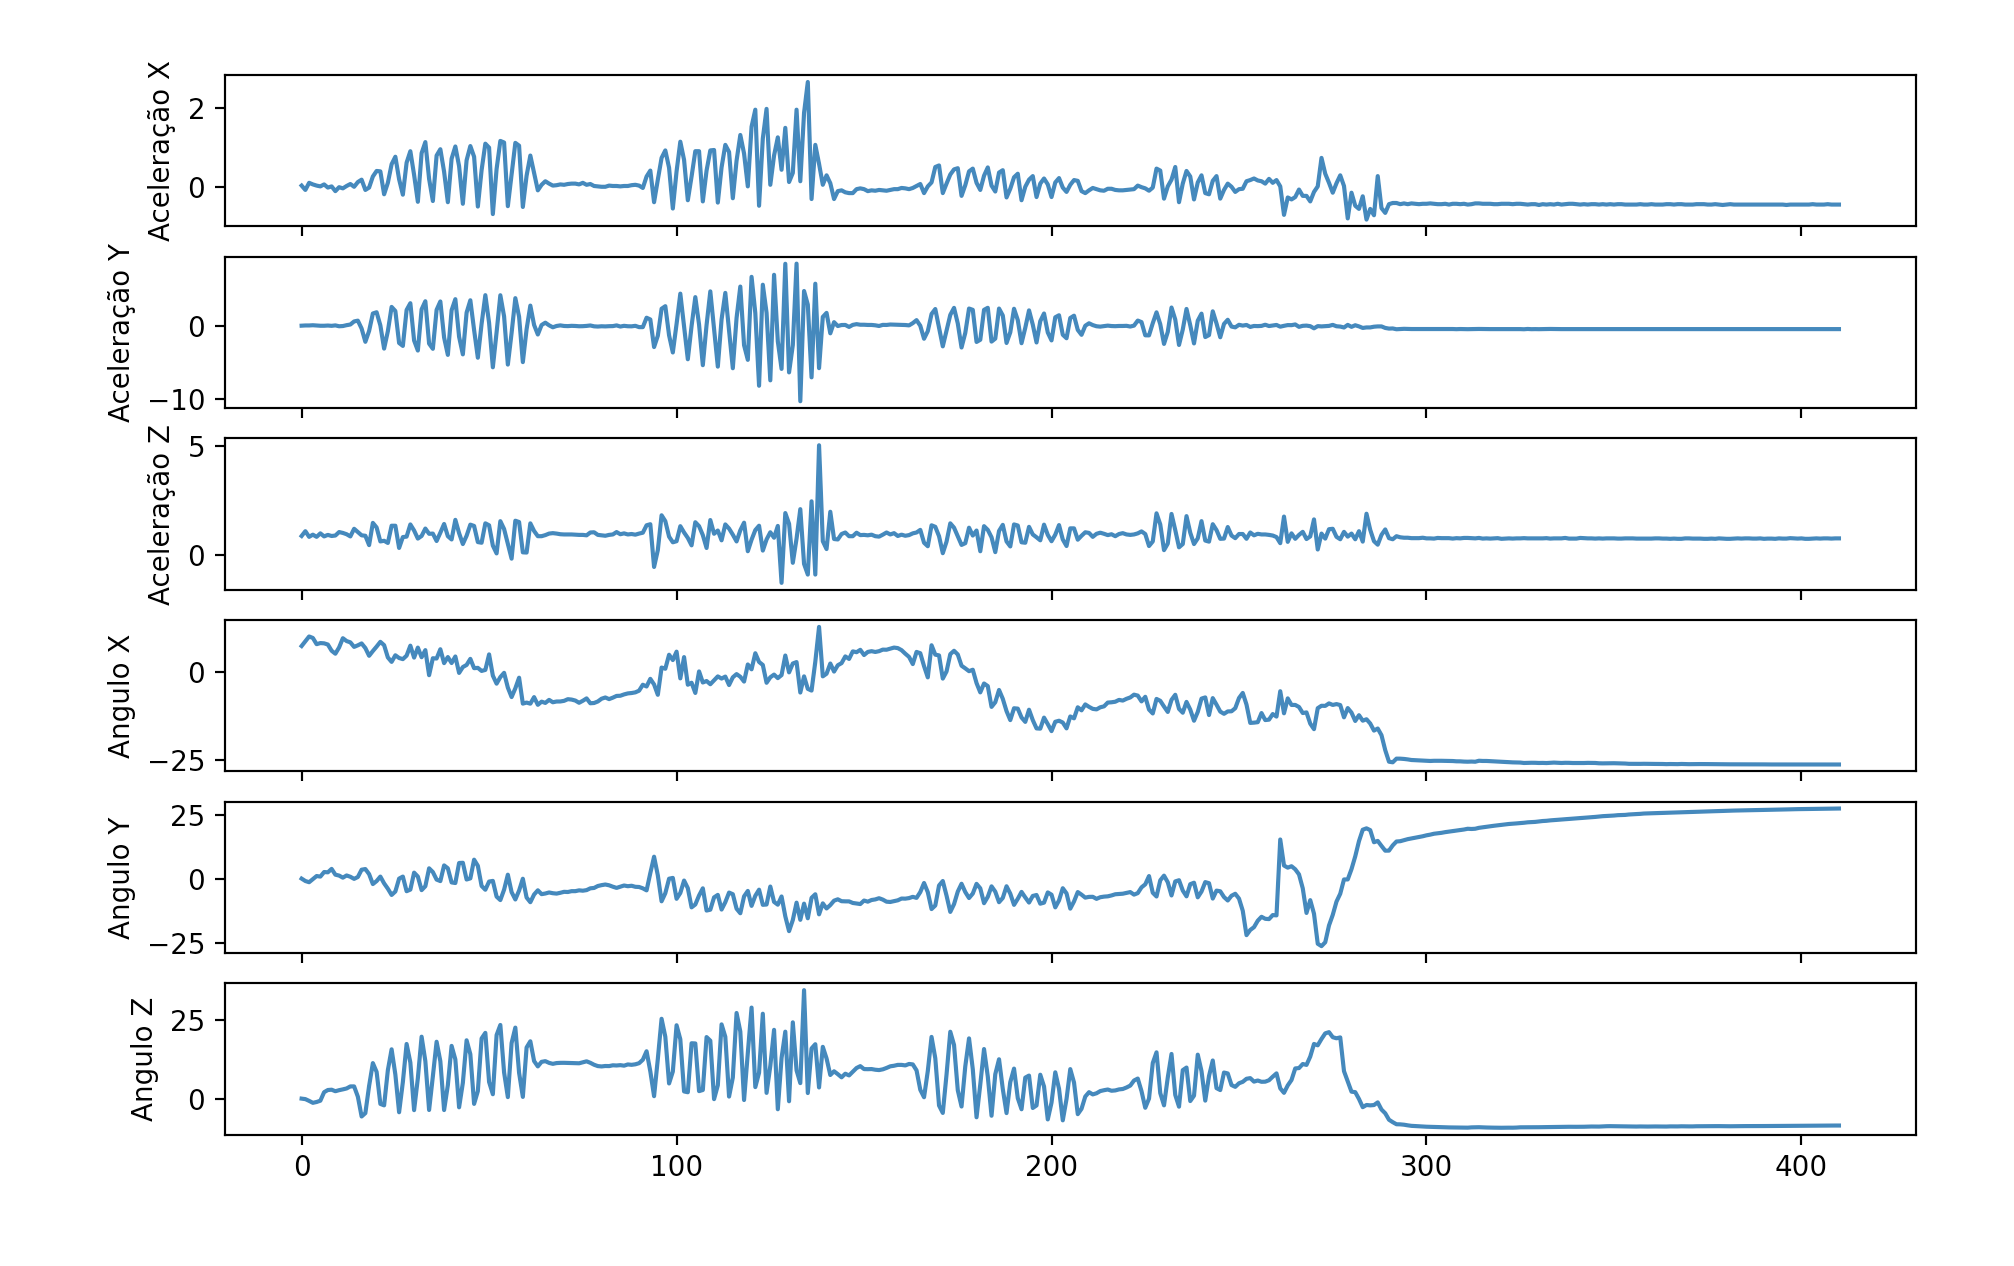
\includegraphics[width=7cm]{images/VibracaoY.png}
    \label{img2}
    \caption{Vibração no eixo Y}
\end{figure}

\begin{figure}[H]
    \center
    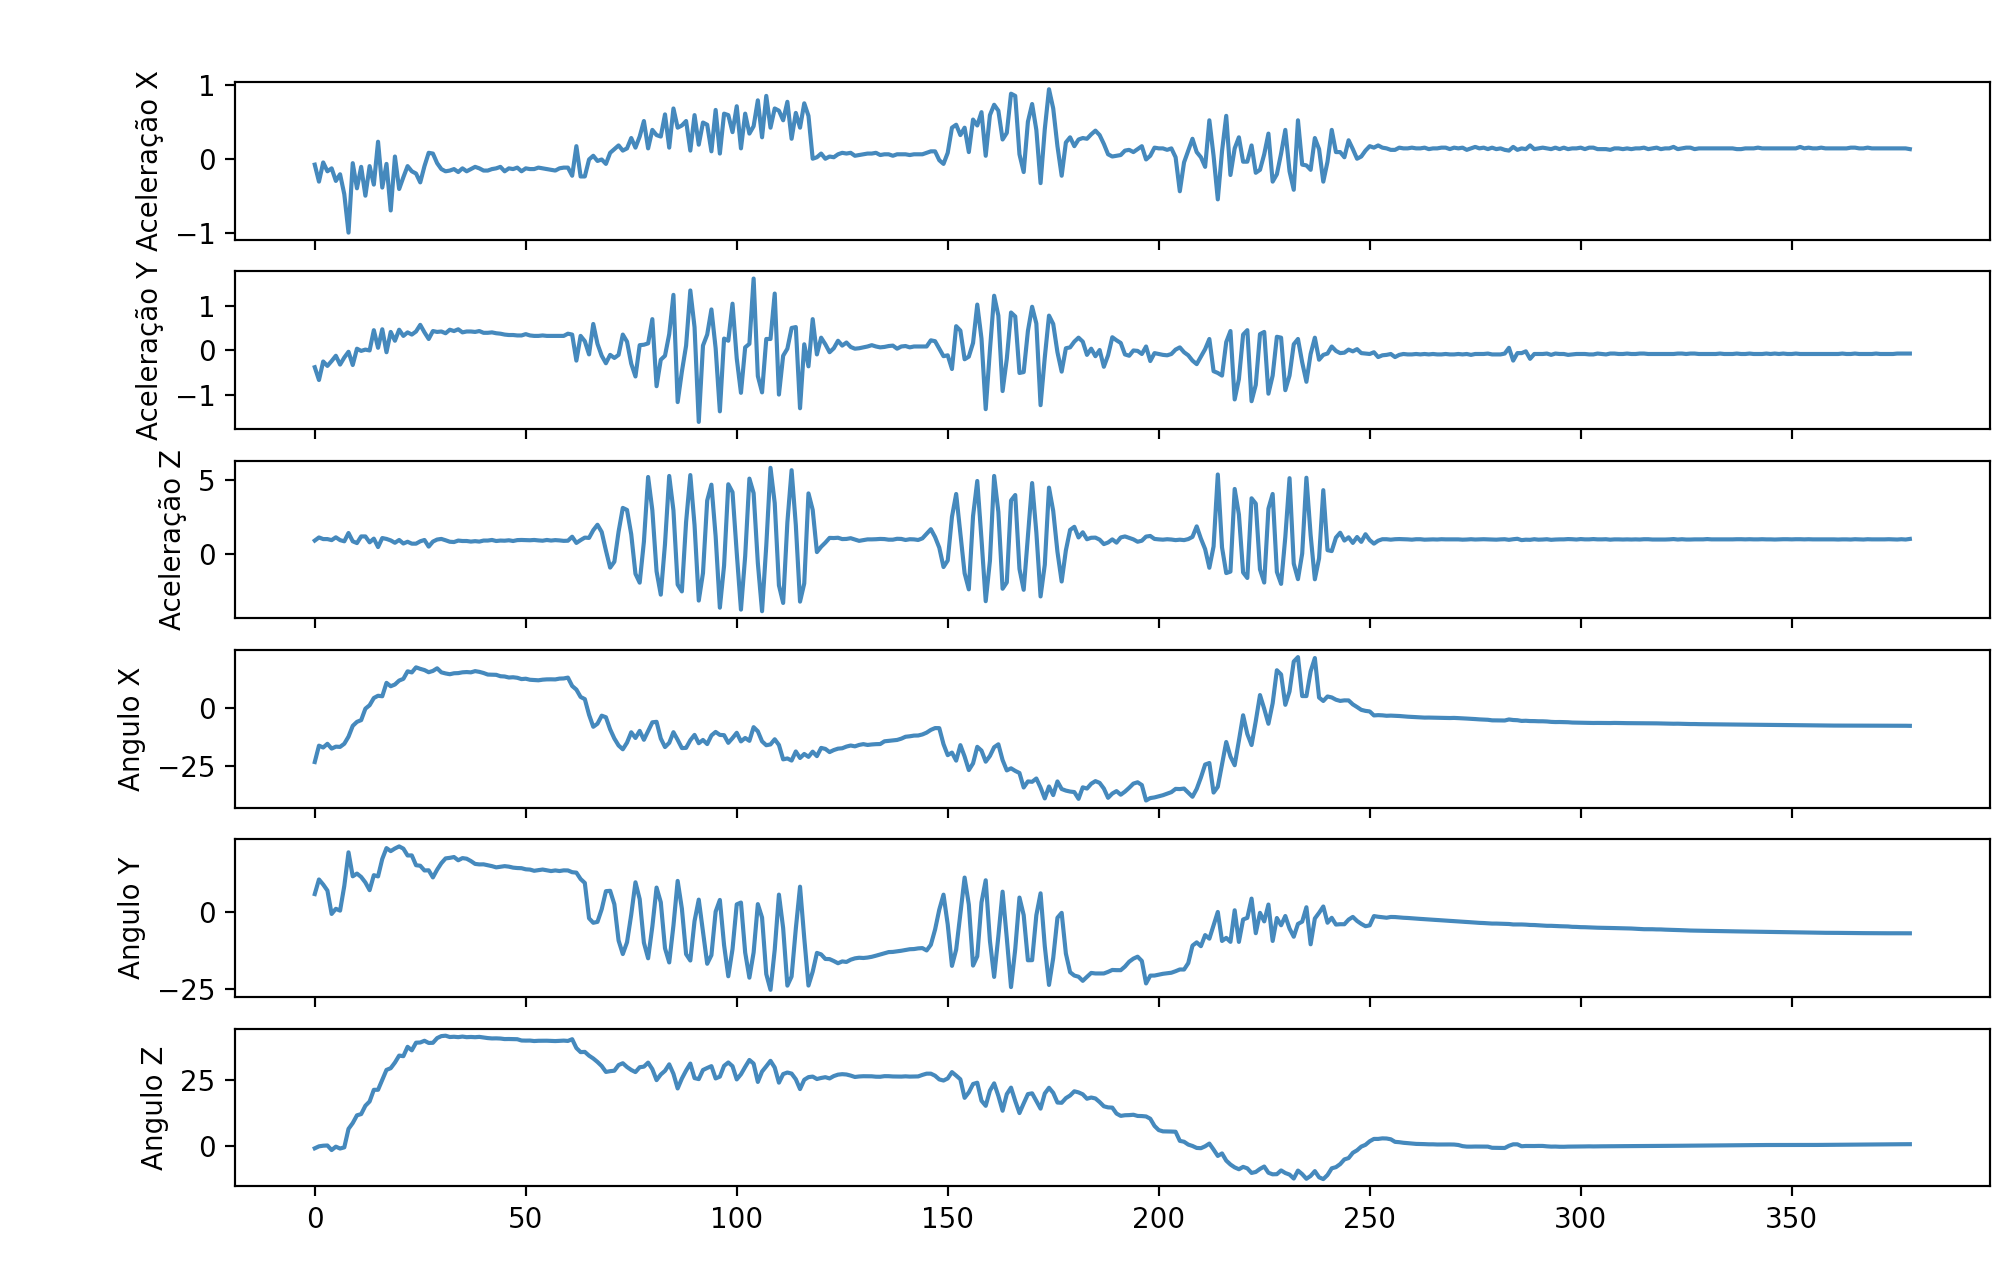
\includegraphics[width=7cm]{images/VibracaoZ.png}
    \label{img3}
    \caption{Vibração no eixo Z}
\end{figure}

\begin{figure}[H]
    \center
    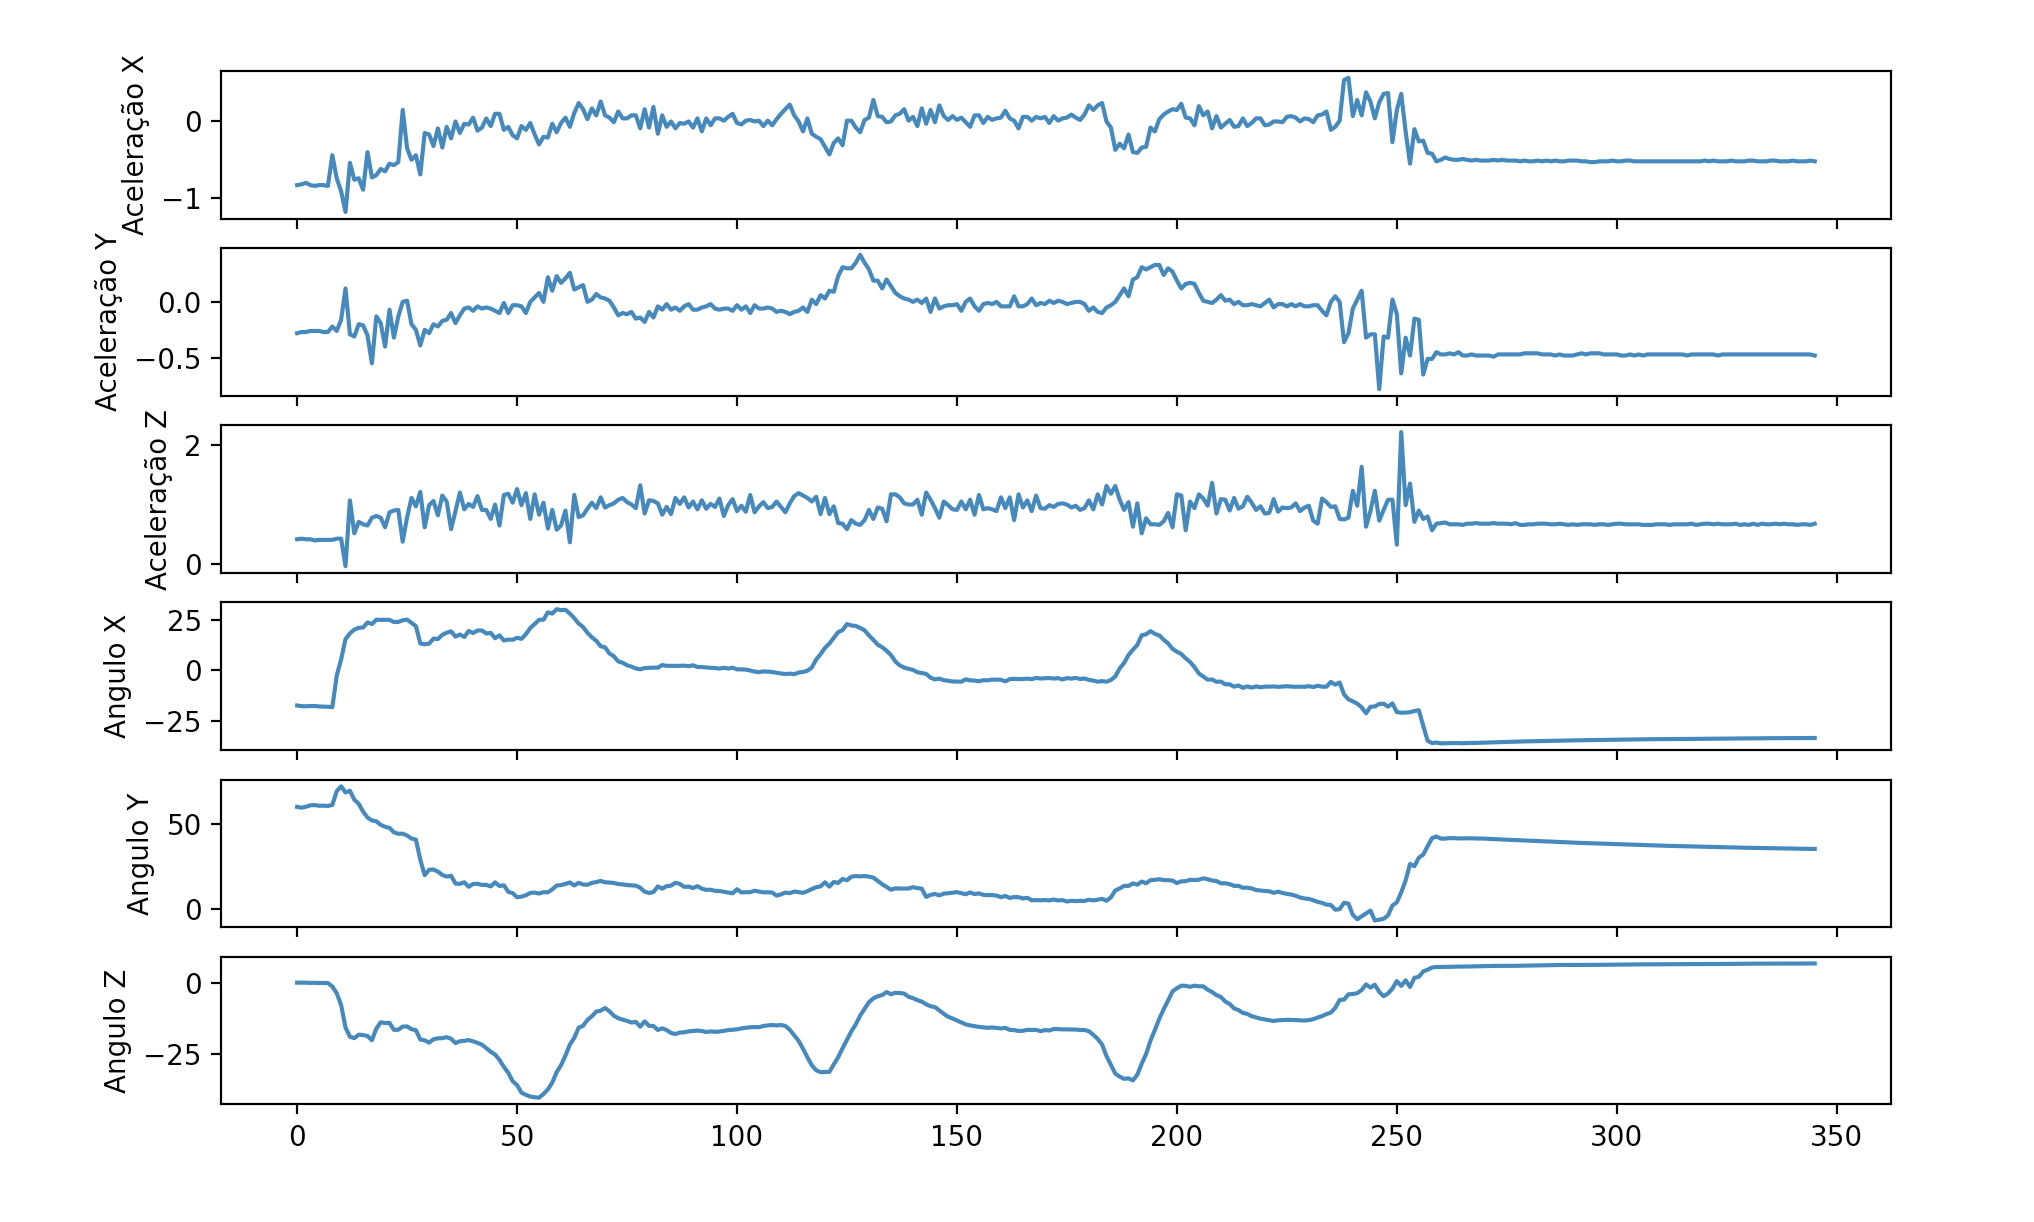
\includegraphics[width=9cm]{images/CirculoZ.png}
    \label{img4}
    \caption{Movimento circular no eixo Z}
\end{figure}

\begin{figure}[H]
    \center
    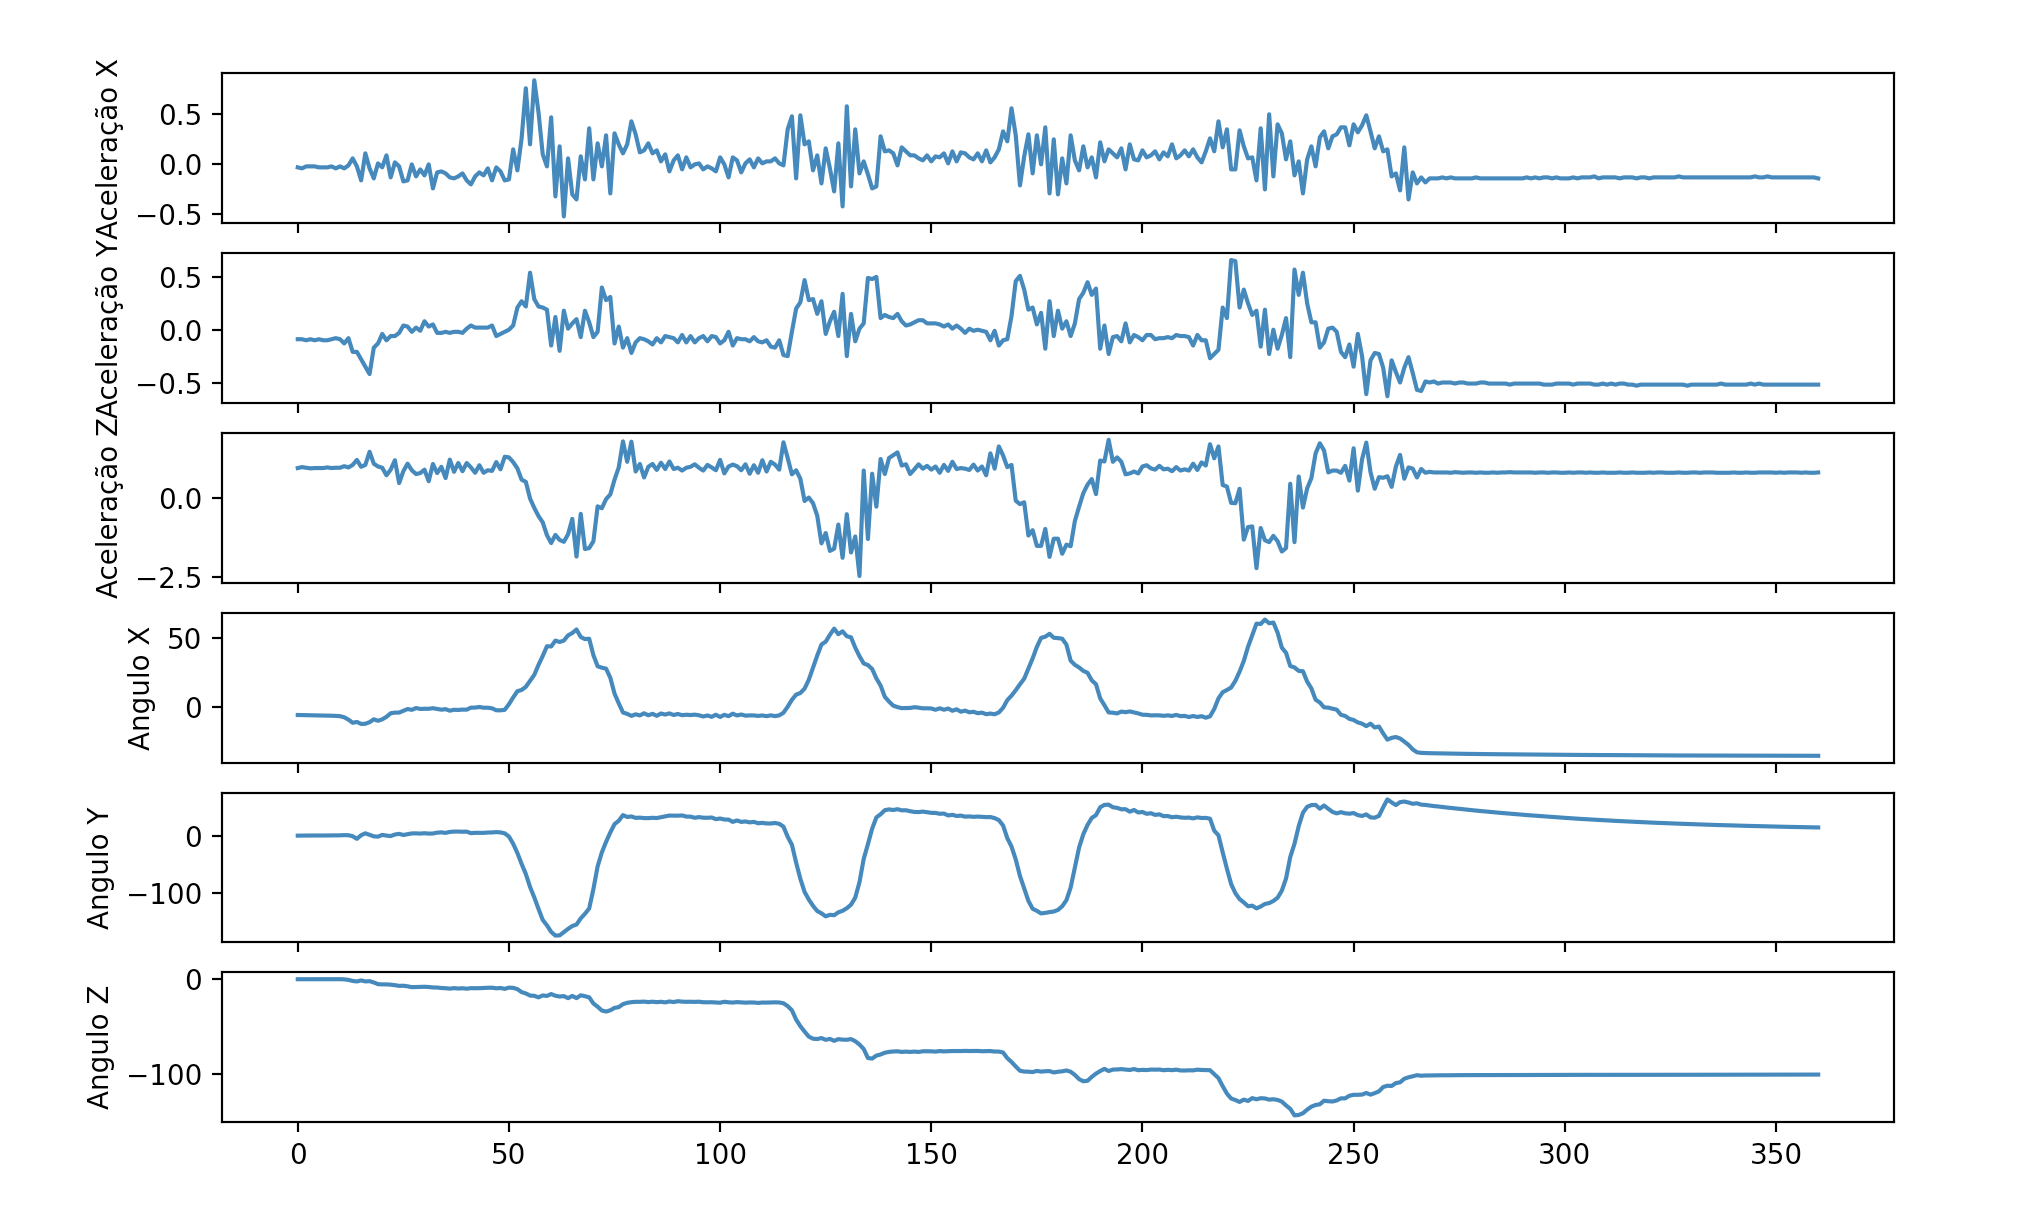
\includegraphics[width=9cm]{images/GiraeVoltaY.png}
    \label{img5}
    \caption{ Gira e Volta no eixo Y }
\end{figure}




\subsection*{3.2 Tratamento dos dados recolhidos}

Primeiramente foi classificado cada comportamento de curva de acordo com seu 
respectivo movimento associado.

Com isso resultamos com um arquivo csv onde cada linha é um valor amostrado no tempo e 
contendo as seguintes colunas:

- AccX (aceleração no eixo X)

- AccY (aceleração no eixo Y)

- AccZ (aceleração no eixo Z)

- AngX (rotação no eixo X)

- AngY (rotação no eixo Y)

- AngZ (rotação no eixo Z)

- Class (classificação do movimento)

Abaixo vemos uma amostra de cada tipo de movimento classificado.

\begin{figure}[H]
    \center
    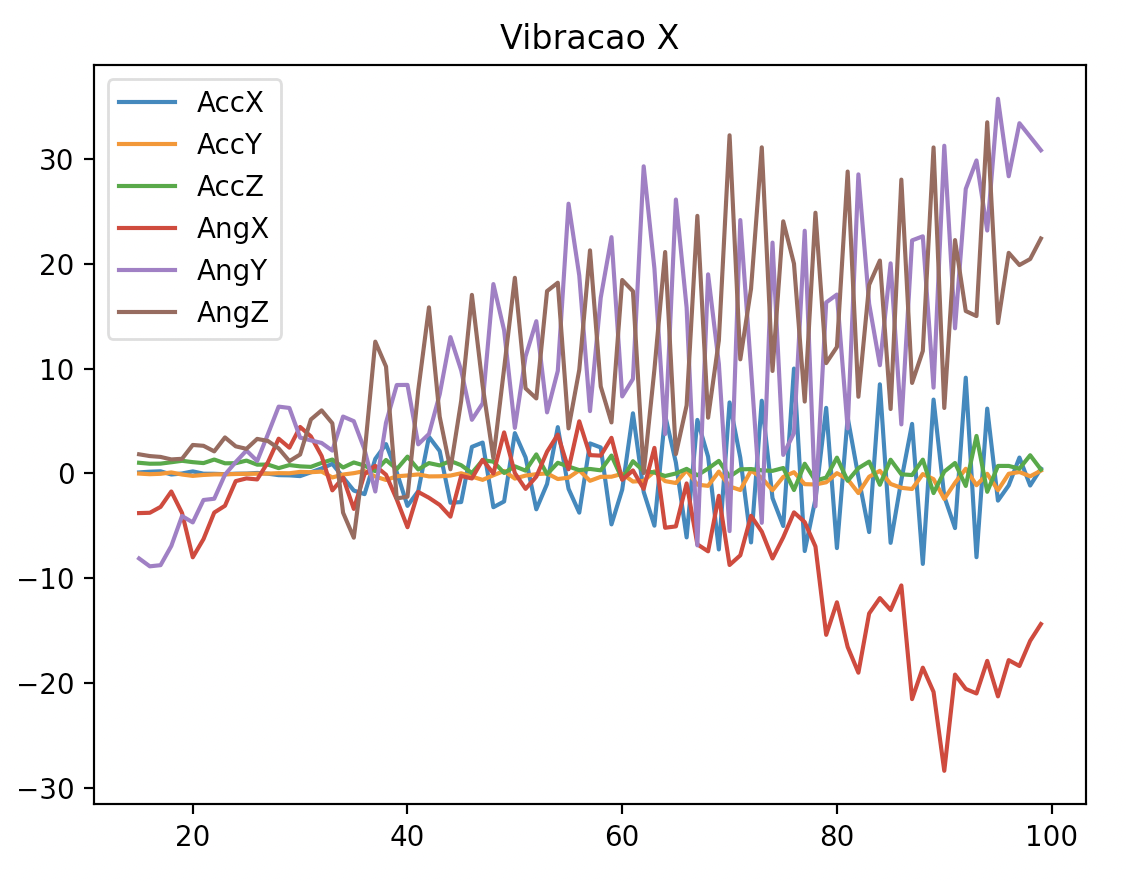
\includegraphics[width=6cm]{images/sampleVibracaoX.png}
    \caption{ sample VibracaoX }
\end{figure}
\begin{figure}[H]
    \center
    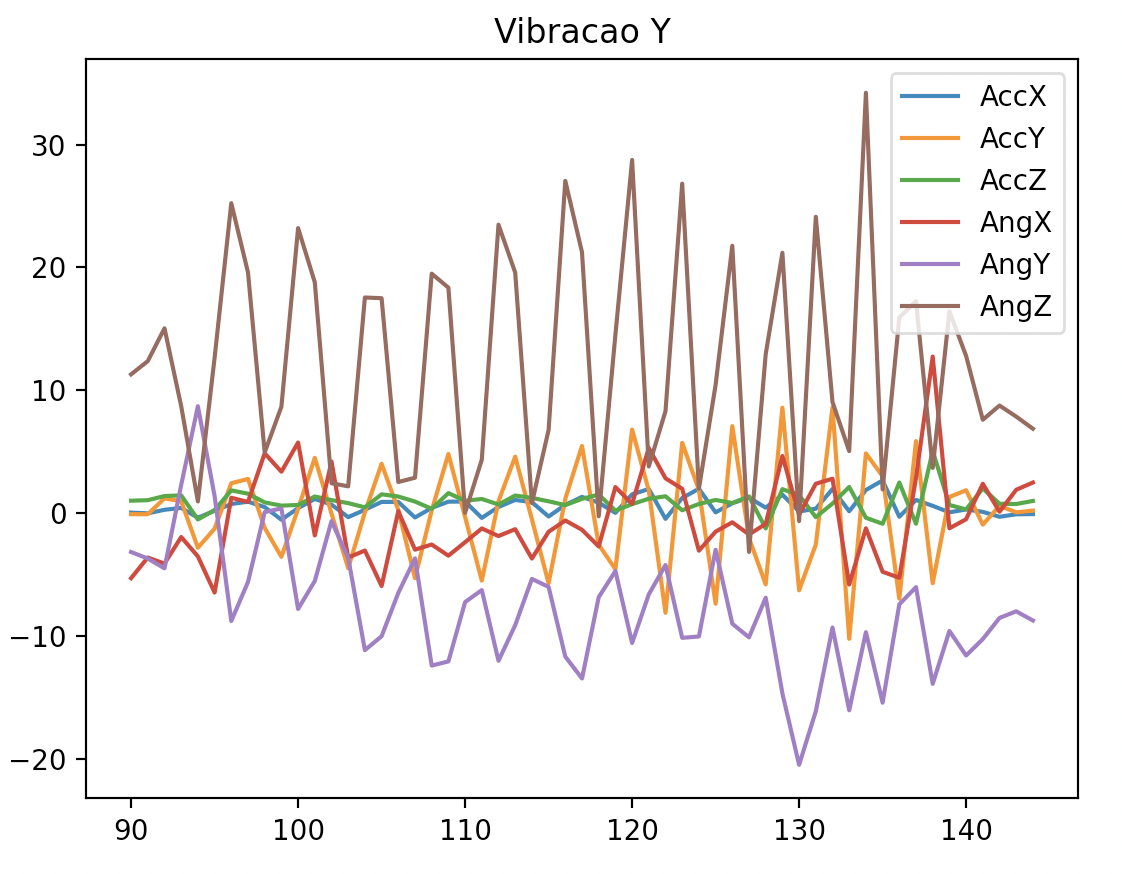
\includegraphics[width=6cm]{images/sampleVibracaoY.png}
    \caption{ sample VibracaoY}
\end{figure}
\begin{figure}[H]
    \center
    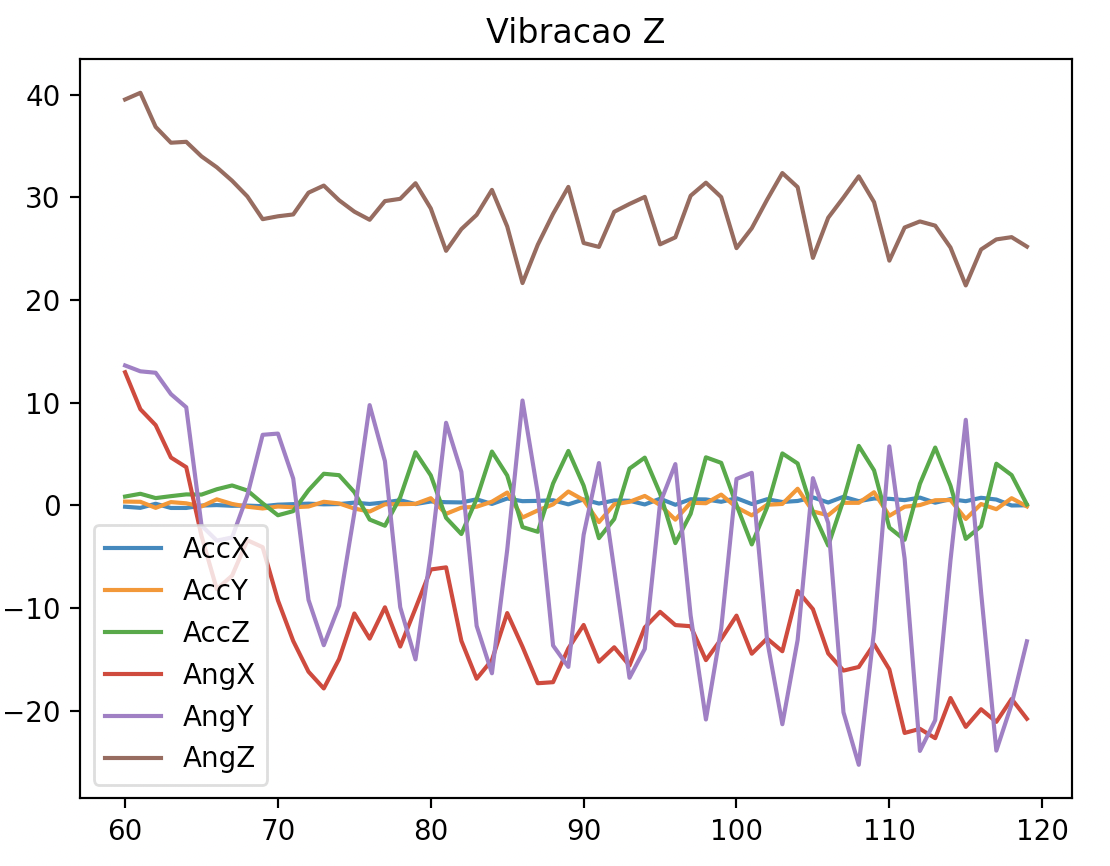
\includegraphics[width=6cm]{images/sampleVibracaoZ.png}
    \caption{ sample VibracaoZ}
\end{figure}
\begin{figure}[H]
    \center
    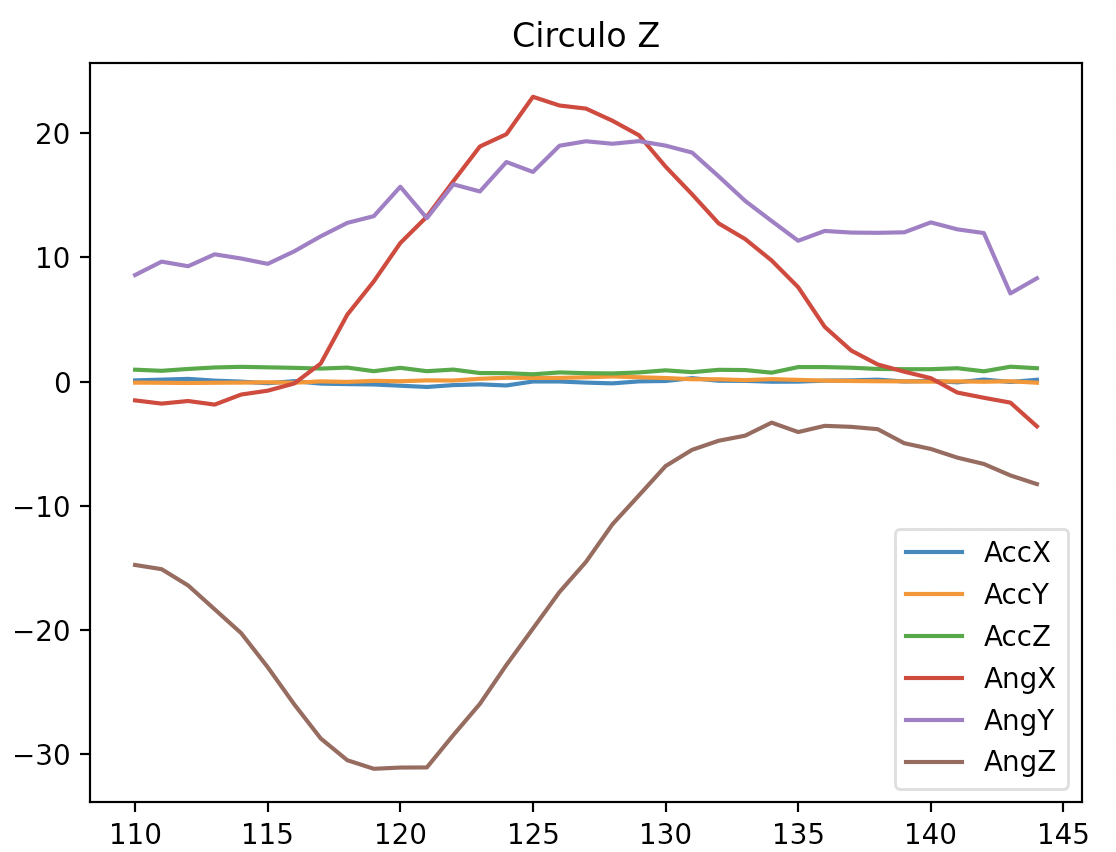
\includegraphics[width=6cm]{images/sampleCirculoZ.png}
    \caption{ sample CirculoZ }
\end{figure}
\begin{figure}[H]
    \center
    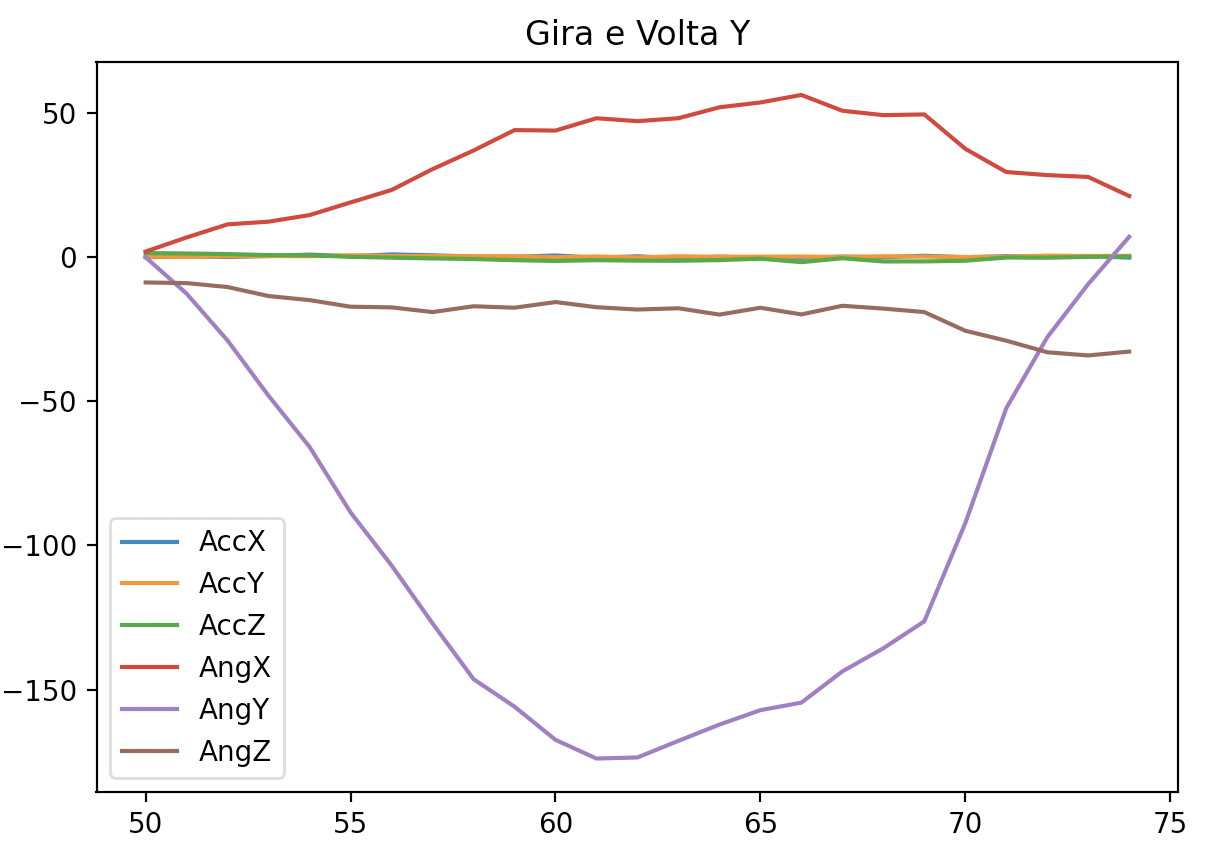
\includegraphics[width=6cm]{images/sampleGiraeVoltaY.png}
    \caption{ sample GiraeVoltaY }
\end{figure}
\begin{figure}[H]
    \center
    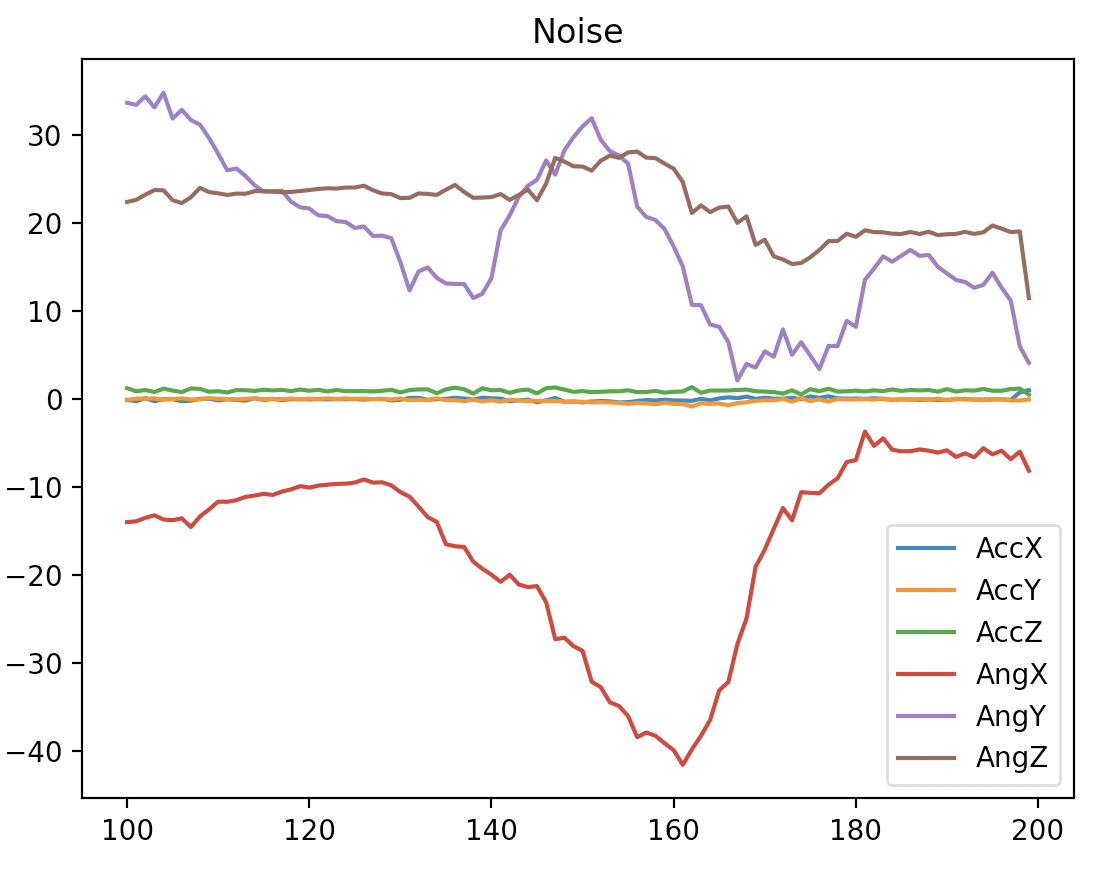
\includegraphics[width=6cm]{images/sampleNoise.png}
    \caption{ sample Noise }
\end{figure}
\begin{figure}[H]
    \center
    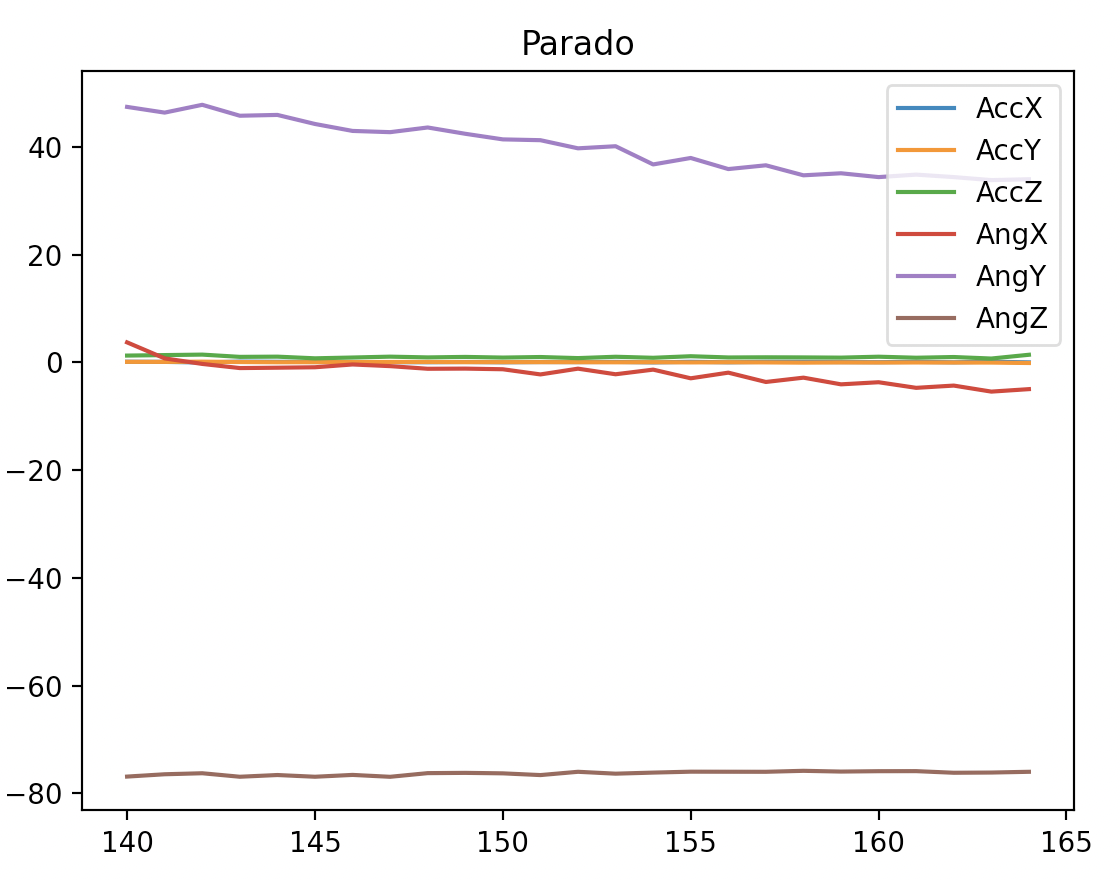
\includegraphics[width=6cm]{images/sampleParado.png}
    \caption{ sample Parado }
\end{figure}

Analisando visualmente já podemos perceber que:

- sinais com maior amplitude alta e frequência alta tendem a ser movimentos de vibração.
Definindo qual eixo temos uma amplitude maior que as demais sabemos qual eixo o movimento foi destinado.

- sinais com amplitude alta em baixas frequências tendem a ser movimento de envolvem rotação.
Definindo o formato da onda conseguimos diferenciar movimento de GiraeVolta de movimentos de Circulo.

- Sinais estáveis definem se o objeto está parado. De acordo com seus valores também podemos saber a posição de repouso.

- Sinais ruidosos são bem comuns em sensores MEMS e por isso não podem ser associados à algum tipo de movimento.




\subsection*{3.2 Análise estatística dos dados}

Primeiramente analisei a distribuição de amostras que temos.
Podemos ver no gráfico de Figura 14 que essa distribuição está desbalanceada.
Temos mais amostras de movimento parado. Além disso temos poucos dados para fazer
um modelo de inferências. Por esse motivo, mais dados serão gerados e classificados na próxima etapa.
Além disso, podemos aplicar técnicas de Undersampling, Oversampling e SMOTE\footcite[]{SMOTE: Synthetic Minority Oversampling Technique}.

\begin{figure}[H]
    \center
    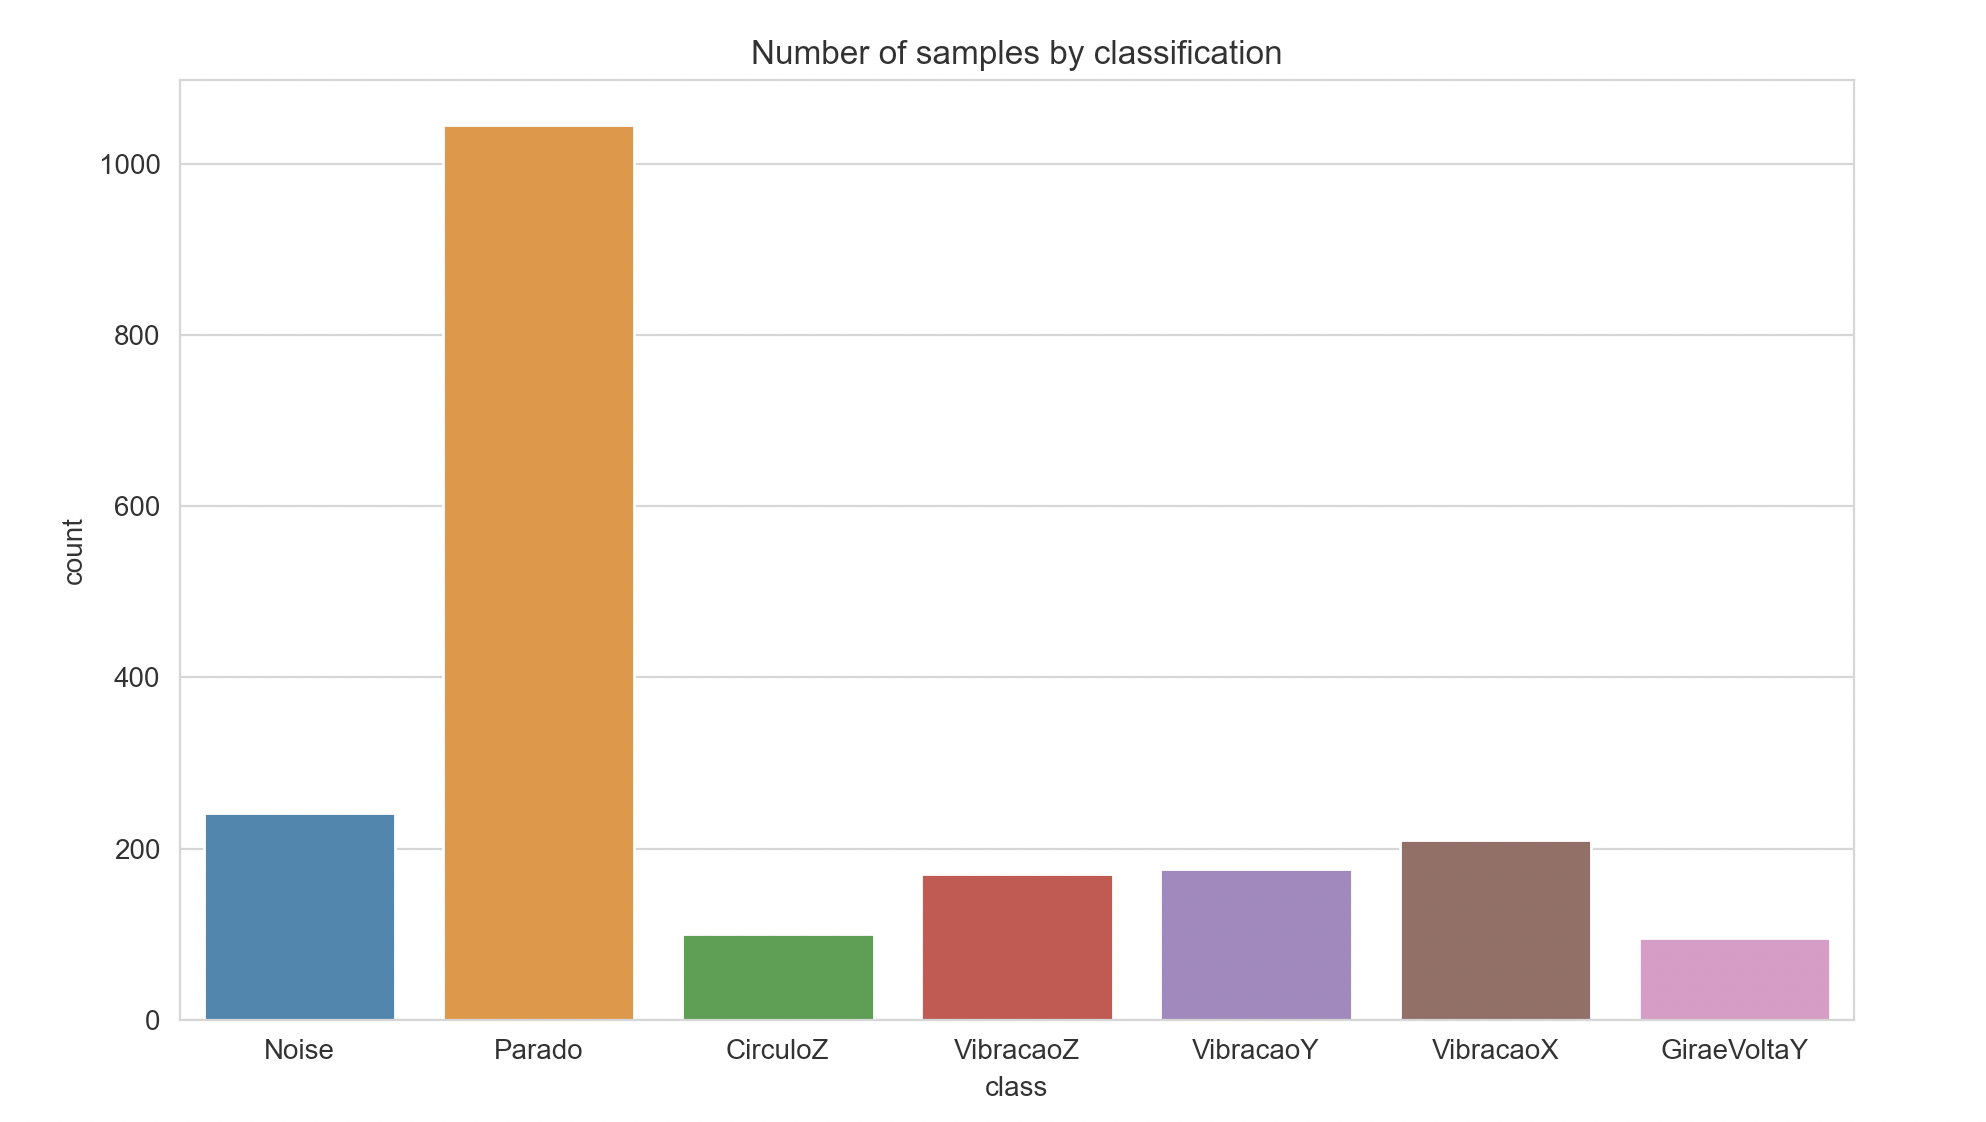
\includegraphics[width=9cm]{images/sampleDistribution.png}
    \caption{ sample Distribution }
\end{figure}

Também foi realizado a distribuição de densidade dos dados em cada eixo do sensor 
para todos os movimentos em questão.

As Figuras 15, 16 e 17 representam os dados recolhidos nos eixos do acelerômetro.
Nelas vemos que o movimento de vibração nos eixos correspondentes apresentam dados mais distribuidos.


\begin{figure}[H]
    \center
    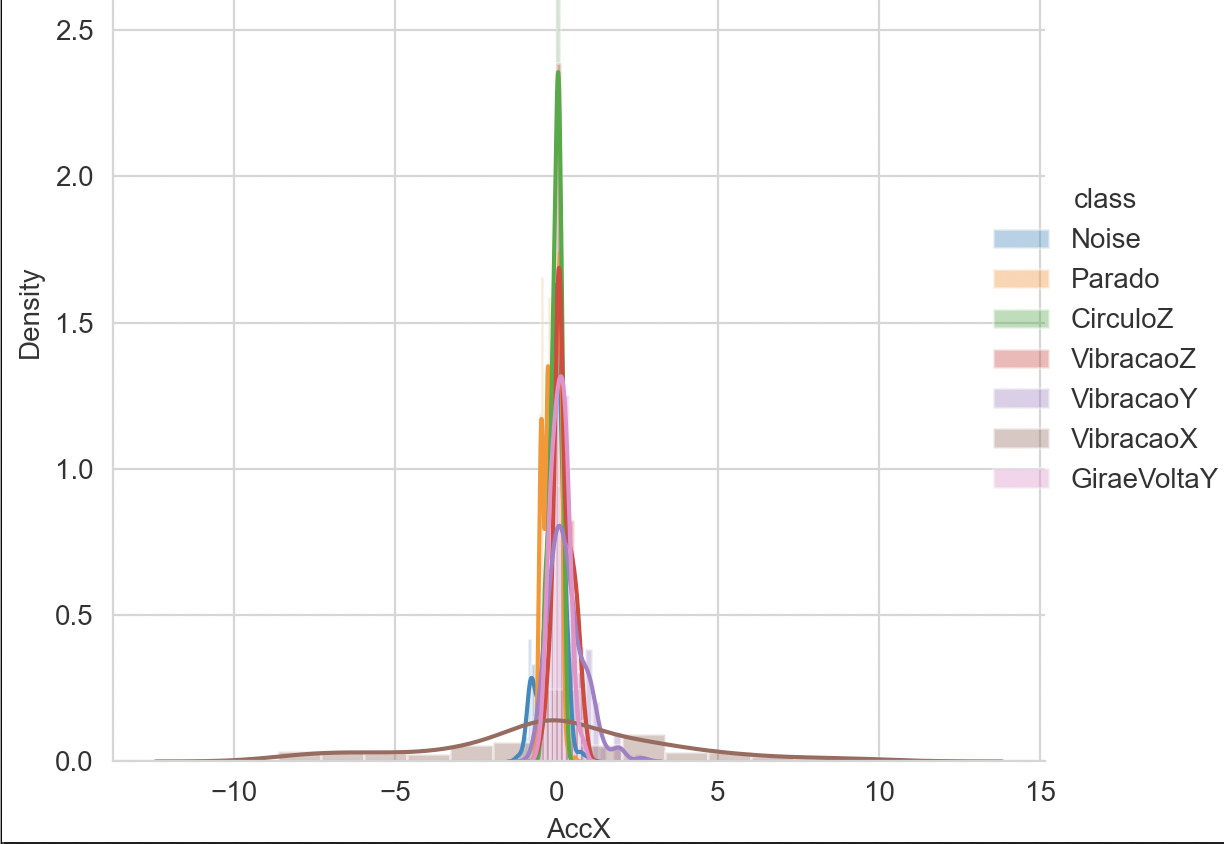
\includegraphics[width=7cm]{images/AccXdistribution.png}
    \caption{ AccX distribution }
\end{figure}
\begin{figure}[H]
    \center
    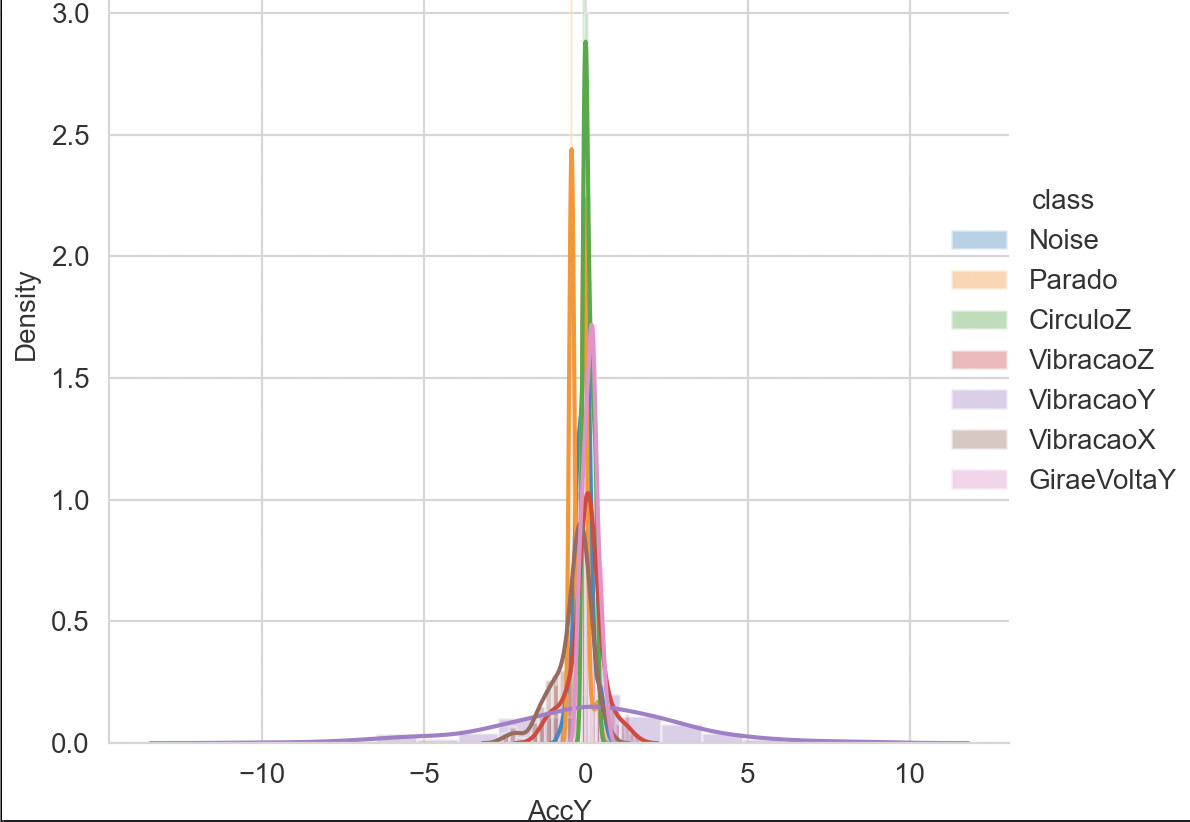
\includegraphics[width=7cm]{images/AccYdistribution.png}
    \caption{ AccY distribution }
\end{figure}
\begin{figure}[H]
    \center
    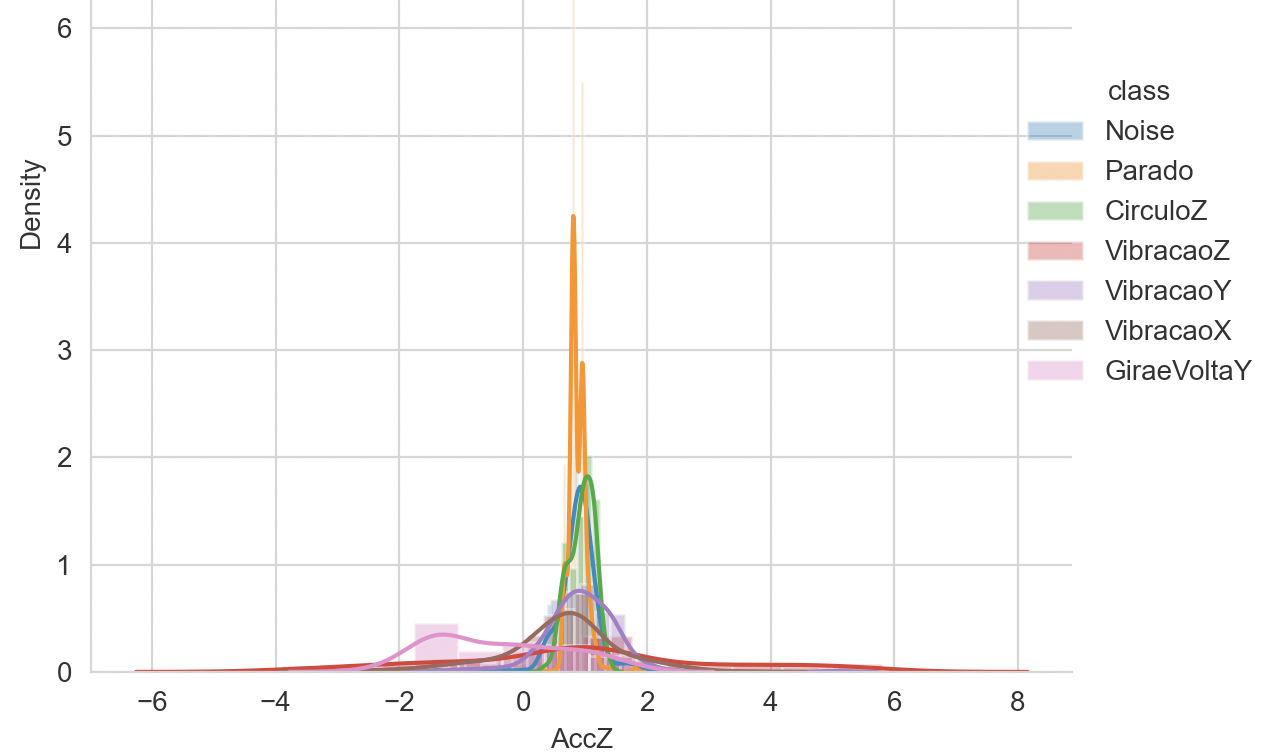
\includegraphics[width=7cm]{images/AccZdistribution.png}
    \caption{ AccZ distribution }
\end{figure}

As Figuras 18, 19 e 20 representam os dados recolhidos nos eixos do giroscópio.
Podemos ver que nos dados desse sensor temos maior separabilidade entre os movimentos de rotação.

\begin{figure}[H]
    \center
    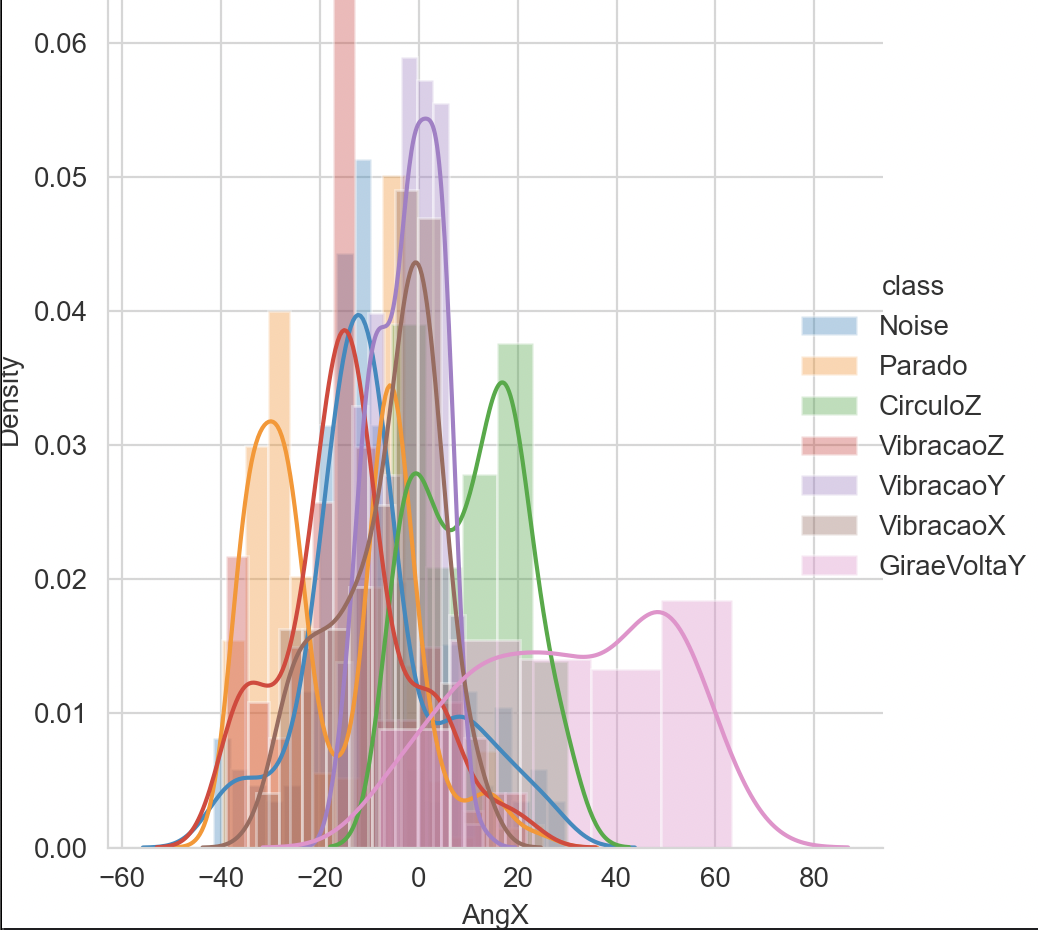
\includegraphics[width=5cm]{images/AngXdistribution.png}
    \caption{ AngX distribution }
\end{figure}
\begin{figure}[H]
    \center
    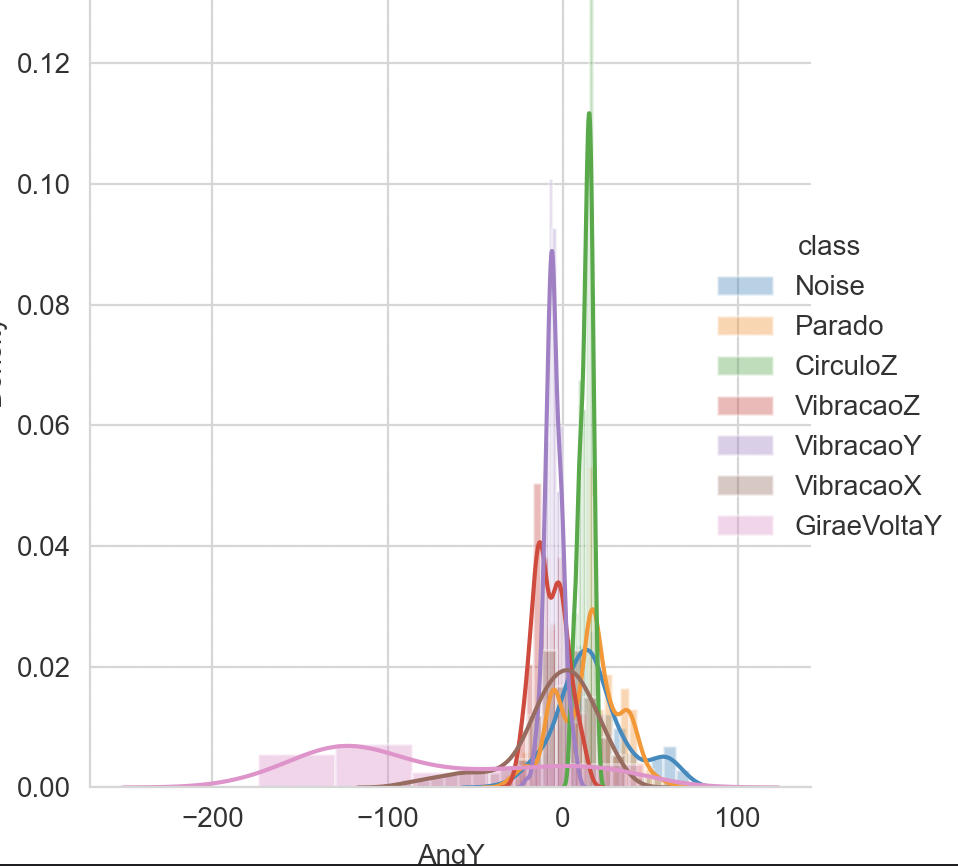
\includegraphics[width=5cm]{images/AngYdistribution.png}
    \caption{ AngY distribution }
\end{figure}
\begin{figure}[H]
    \center
    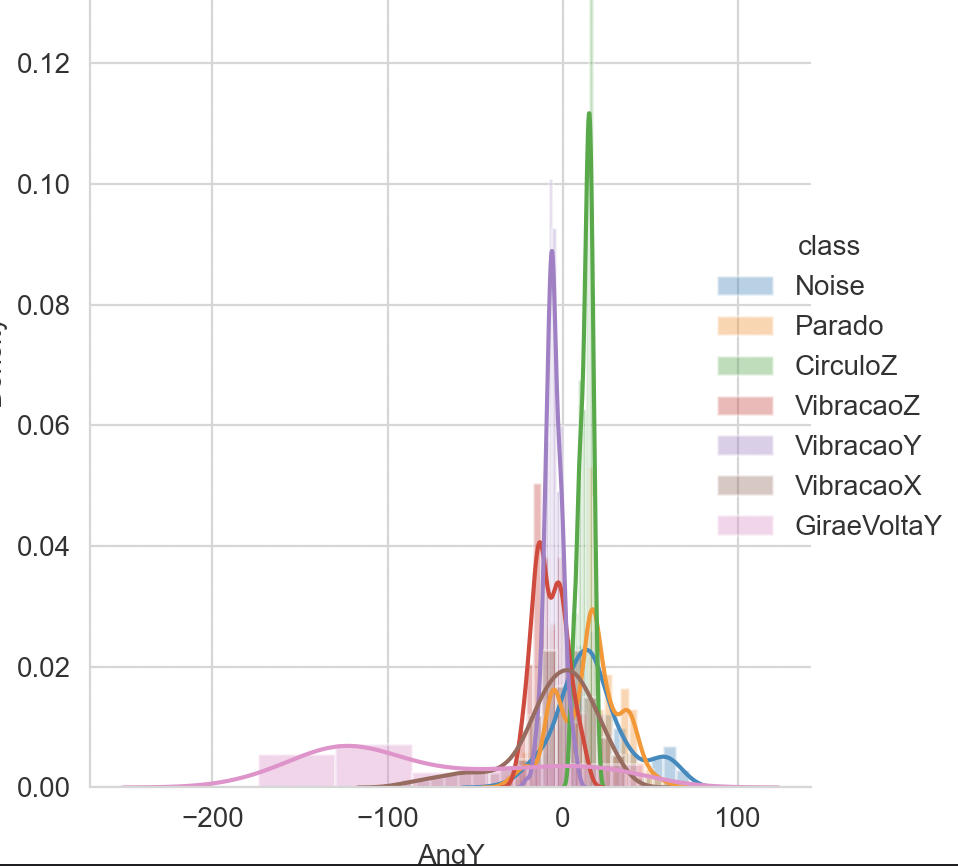
\includegraphics[width=5cm]{images/AngYdistribution.png}
    \caption{ AngY distribution }
\end{figure}

\subsection*{3.3 Data Transformation}

Nessa etapa os dados foram reorganizados em listas de janelas de tempo (''windowing''). Isso porque um movimento não consegue ser
detectado com apenas as informações adquiridas em uma amostra de tempo, mas sim em uma janela de amostras.
Por esse motivo foram agregados 50 amostras em uma lista de valores e sua respectiva classificação. Essa transformação foi implementada de forma não discreta entre os dados,
ou seja, cada janela de tempo terá dados da janela de tempo anterior também.



